\chapter{Abordagem}
\label{sec:abordagem}

Este capítulo tem como principal objectivo descrever a metologia adoptada e ainda apresentar o planeamento do projecto tal como os desvios relativamente ao mesmo. Por fim será apresentada uma analise dos riscos associados ao projecto que poderão tem um impacto negativo no plano de desenvolvimento. Este conjunto de passos foca-se em atingir um produto final bem estruturado e funcional, utilando boas práticas de desenvolvimento de software


\section{Metodologia}
\label{metodologia}

A metodologia de desenvolvimento do projecto adoptada foi uma metodologia fortemente baseada em SCRUM\cite{scrum}, que será descrita (i. e. os aspectos mais importantes) nesta secção. Esta é a metodologia utilizada pela 10.digital e tendo em conta que esta metodologia ágil se encaixa perfeitamente nas necessidades do projecto, estes foram os factores decisivos para a escolha da mesma. 

Líder em desenvolvilmento àgil, o SCRUM, é uma metodologia apontada para projectos com foco em trazer valor ao cliente de forma incremental, através de iterações de curta duração, chamadas Sprints. Esta metodologia possibilita também a abordagem de problemas complexos de forma produtiva, prioritorizar tarefas durante a fase de desenvolvimento e ainda facilita a inclusão de novas funcionalidades sempre que ncessário. Desta forma o SCRUM proporciona uma gestão flexível do projecto e permite realizar pequenas alterações no planeamento, sem necessidade de interromper o desenvolvimento.

\subsection{Intervenientes}

Um aspecto determinante para o sucesso do SCRUM é o trabalho em equipa. Tipicamente nesta metodologia existem três papeis pré-definidos: \textit{Product Owner}, \textit{Scrum Master} e \textit{Scrum Team}.

O \textbf{\textit{Product Owner}} representa o cliente e é responsável por transmitir a visão do produto, ou por outras palavras, é responsável por maximizar o valor do produto e o trabalho da equipa de desenvolvimento (i. e. \textit{Scrum Master}). É responsável por organizar e priorizar as taferas no \textit{product backlog}.

O \textbf{\textit{Scrum Master}} tem um papel fundamental no desempenho da \textit{Scrum Team}. É responsável por garantir o cumprimento das práticas do SCRUM, ajudar e orintar a \textit{Scrum Team} especialmente nas dificuldades que vão surgindo ao longo do projedcto e, de forma gradual (i. e. respeitando as \textit{Sprints}), apresentar o trabalho realizado ao \textit{Product Owner}.

A \textbf{\textit{Scrum Team}} representa os elementos que constituem a equipa de desenvolvimento que com a orientação do \textit{Scrum Master}, monitorizam o trabalho que vai sendo feito e assim conseguir cumprir com as \textit{sprints backlog}. A \textit{Scrum Team} deve ser autónomae organizada.

\subsection{Processo}

O Desenvolviemento começa assim que o \textit{product backlog} estiver concluído e detalhado pelo \textit{Product Owner}. O \textit{product backlog} representa a lista requisitos necessários para atingir o produto final. 

Depois de definido o \textit{product backlog}, o \textit{Scrum Master}, juntamente com a \textit{Scrum Team} reunem e definem o tempo para cada \textit{Sprint}. Tipicamente as \textit{Sprints} tem duração entre 1 a 4 semanas e no final das mesmas é apresentado o trabalho realizado pela \textit{Scrum Team}. No inicio de cada \textit{Sprint} é criada a \textit{Sprint Backlog}. Na \textit{Sprint Backlog} é estipulado o conjunto de funcionalidades/tarefas a realizar durante a \textit{Sprint}. Na 10.digital a variável da velocidade não é implementada na \textit{Sprint Backlog}.

No inicio de cada dia é realizada a \textit{Daily Scrum}, uma reunião que tem uma duração de 15$\pm$5 minutos, onde, de forma informal, são discutidas as tarefas que devem ser implementadas nesse dia, o ponto de situação do projeto relativo ao dia anterior e caso haja algum impasse ou dificuldade na realização de alguma tarefa, imediatamente após a reunião (i. e. assim que possível) tentasse arranjar uma solução para o mesmo. 

No final de cada \textit{Sprint} há uma reunião (\textit{Sprint Review}) para verificar as tarefas que foram realizadas. Durante a reunião a \textit{Scrum Team} apresenta as novas funcionalidades implementadas para os restantes participantes que podem ser \textit{Product Owner}, \textit{Scrum Master}, clientes e outros colegas de trabalho. 

A Figura \ref{fig:scrum} sumariza todo o processo descrito anteriormente.



\begin{figure}[ht!]
	\begin{center}
		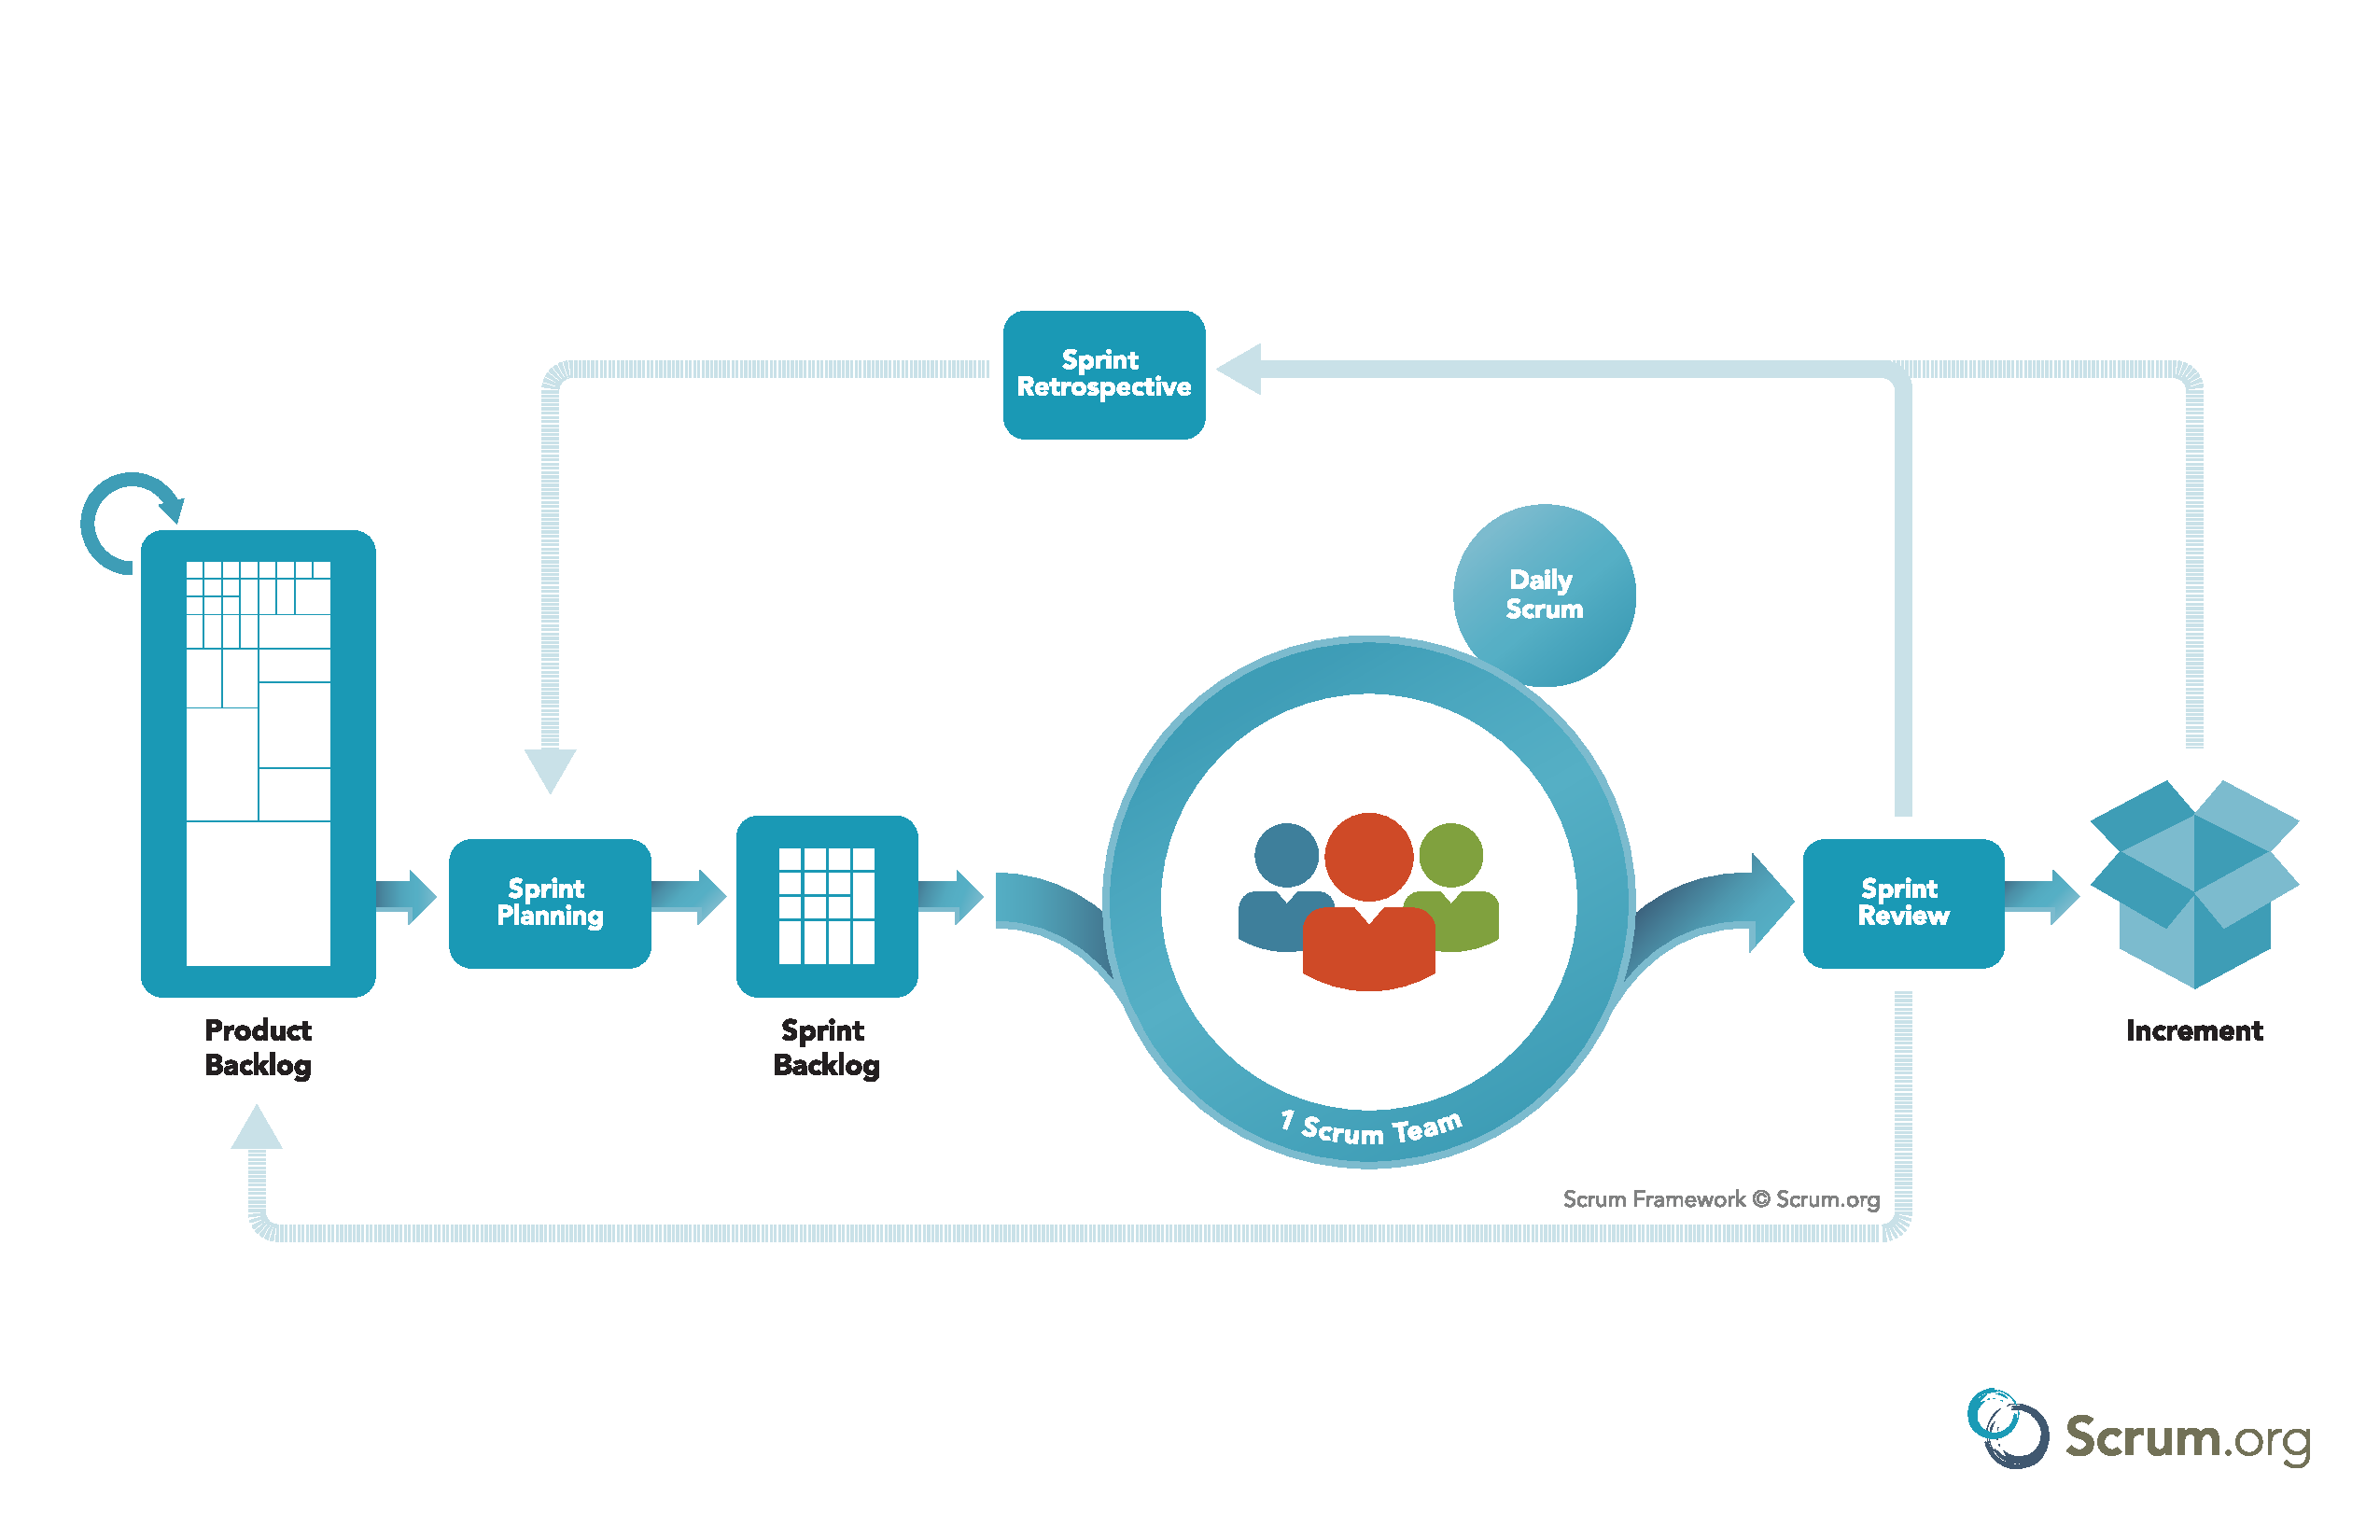
\includegraphics[width=1\textwidth]{img/scrum.pdf}
		\caption{Scrum Framework\cite{scrumimg}}
		\label{fig:scrum}
	\end{center}
\end{figure}

\newpage

\section{Planeamento}
\label{planeamento}

Nesta secção será apresentado o plano de estágio do primeiro e segundo semestre, através de diagramas de Gantt.  De seguida será exposto o desvio temporal em relação ao planeado e por fim serão brevemente detalhados os artefactos (i. e. \textit{Sprint Backlog}) da metologia SCRUM.

Como foi referido no Capítulo \ref{sec:introducao}, este documento expõe o trabalho realizado neste projecto durante o ano lectivo, por isso, apenas será exposto o desenvolvimento do \textit{back-end} da plataforma de inbound marketing. Dito isto, a equipa de desenvolvimento será composto por multiplas pessoas sendo que cada um terá a sua função distinta.
No seguimento do ponto anterior, os cargos de cada interveniente no projecto são:
\begin{itemize}
	\item[--] \textbf{\textit{Product Owner}}: Eng. Pedro Beck
	\item[--] \textbf{\textit{Scrum Master}}: Eng. Pedro Beck
	\item[--] \textbf{\textit{Scrum Team}}: 
	\subitem  \textit{Front-End Developer} - Por Definir
	\subitem  \textit{Back-End Developer} - Bruno Grifo
	\subitem  \textit{Back-End Developer \acrshort{tcg}} - Eng. Pedro Beck
\end{itemize}

É ainda de referir que, no primeiro semestre, o Mestre João Oliveira realizou o papel de co-orientador na empresa e teve um impacto importante na orientação do projecto de tese. 

\begin{figure}[ht!]
	\begin{center}
		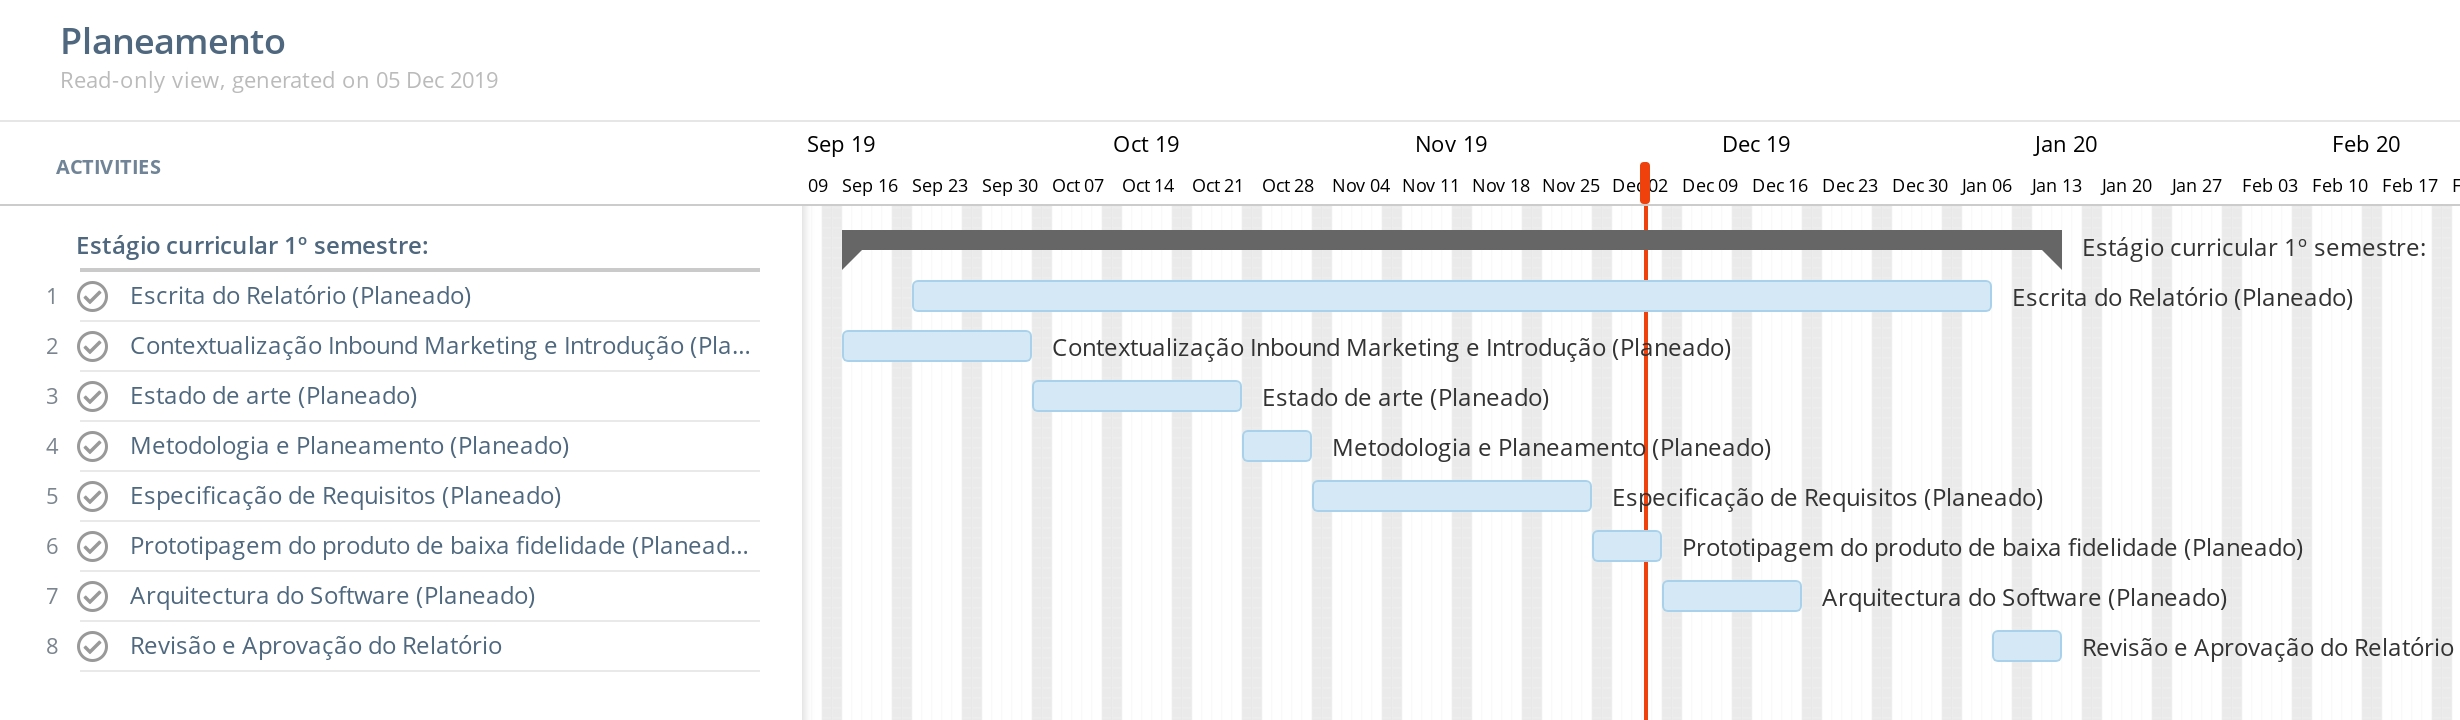
\includegraphics[width=1\textwidth]{img/gantt/semestre1.jpeg}
		\caption{Diagrama de Gantt - Planeamento do 1º semestre}
		\label{fig:gantt1}
	\end{center}
\end{figure}

Representado na Figura \ref{fig:gantt1} temos o plano de estágio relativo ao primeiro semestre. A escrita do relatório intermédio foi divido nas seguintas 6 tarefas principais:
\begin{itemize}
	\item \textbf{Contextualização Inbound Marketing e Introdução}: Tendo em conta a àrea onde o projecto se indice foi realizado um estudo sobre inbound marketing para que me pudesse contextualizar e conseguir compreender as diversas estratégias de inbound. No final da tarefa foi realizada uma apresentação sobre este tema e avaliada pelo co-orientador da empresa, para garantir o nível de conhecimento pretendido. Este estudo foi crucial para desenhar o modelo de negócio do projecto.
	\item \textbf{Estado de Arte}: Nesta tarefa foi feito o levantamento do estar de arte. Foram analisadas várias aplicações/plataformas conconrrentes ou com funcionalidades semelhantes para ganhar um melhor conhecimento sobre o mercado.
	\item \textbf{Metodologia e Planeamento}: Foi feito um estudo interno para perceber ao detalhe como foi adoptada a metodologia SCRUM na empresa.
	\item \textbf{Especificação de Requisitos}: Esta tarefa começou com a elaboração de alguns prototipos de baixa fidelidade e um conjunto de requisitos funcionais. De seguida foi marcada uma reunião com o cliente onde, pegando no trabalho realizado anteriormente, foi feito os devidos ajustes e levantado os restantes requisitos. Foi assim documentado os requisitos não funcionais, funcionais e respectivos casos de uso e ainda as restrições técnicas e de negócios.
	\item \textbf{Prototipagem de produto de baixa fidelidade}: Foi criado um conjunto de protótipos que representam todos as funcionalidades principais da plataforma e de igual forma satisfazem o caso de uso correspondente.
	\item \textbf{Arquitectura de Software}: Nesta tarefa foi projectada a arquitectura a desenvolver no âmbito od estágio.
\end{itemize}

Neste projeto cada sprint dura duas semanas e a sprint meeting é feita no último dia. Em cada sprint meeting estão presentes os estagiários (scrum master e scrum team), os orientadores (product owner) e, sempre que possível, o tutor. Cada estagiário apresenta o que fez durante o sprint, executa o demo das funcionalidades implementadas e partilha as dificuldades encontradas durante o sprint com os restantes. Os orientadores dão feedback, tanto do resultado geral do sprint, como de cada funcionalidade (user story) implementada.


Neste semestre cada \textit{Sprint} tem a duração de 2 semanas e no final da mesma é feita uma reunião de ponto (i. e. \textit{Daily Scrum}), onde estão presentes o \textit{Product Owner}, \textit{Scrum Master}, clientes e outros colegas de trabalho que queiram participar. Nesta primeira fase, no total foram realizadas 7 \textit{Sprints}:

\begin{itemize}
	\item \textbf{\textit{Sprint} \#1}
		\subitem \textbf{Data Início}: 16/09/2019
		\subitem \textbf{Data Fim}: 27/09/2019
		\subitem \textbf{Descrição}: Estudo sobre Inbound Marketing.
	\item \textbf{\textit{Sprint} \#2}
		\subitem \textbf{Data Início}: 28/09/2019
		\subitem \textbf{Data Fim}: 11/10/2019
		\subitem \textbf{Descrição}: Escrita do Capítulo \ref{sec:introducao} e inicio do estudo sobre aplicações/plataformas concorrentes.
	\item \textbf{\textit{Sprint} \#3}
		\subitem \textbf{Data Início}: 12/10/2019
		\subitem \textbf{Data Fim}: 25/10/2019
		\subitem \textbf{Descrição}: Conclusão do estudo de mercado e escrita do Capítulo \ref{sec:estado-arte}.
	\item \textbf{\textit{Sprint} \#4}
		\subitem \textbf{Data Início}: 26/10/2019
		\subitem \textbf{Data Fim}: 08/11/2019
		\subitem \textbf{Descrição}: Escrita do Capítulo \ref{sec:abordagem} e reunião com o cliente para levantamento de requisitos.
	\item \textbf{\textit{Sprint} \#5}
		\subitem \textbf{Data Início}: 09/11/2019
		\subitem \textbf{Data Fim}: 22/11/2019
		\subitem \textbf{Descrição}: Escrita do Capítulo \ref{sec:requisitos}.
	\item \textbf{\textit{Sprint} \#6}
		\subitem \textbf{Data Início}: 23/11/2019
		\subitem \textbf{Data Fim}: 06/12/2019
		\subitem \textbf{Descrição}:  Escrita dos casos de Uso no Anexo \ref{a:cu} e prototipagem do produto de baixa fidelidade no Anexo \ref{a:prototipos}.
	\item \textbf{\textit{Sprint} \#7}
		\subitem \textbf{Data Início}: 06/11/2019
		\subitem \textbf{Data Fim}: 20/12/2019
		\subitem \textbf{Descrição}: Projeção da arquitectura e escrita do Capítulo \ref{sec:arquitetura}
\end{itemize}

\begin{figure}[ht!]
	\begin{center}
		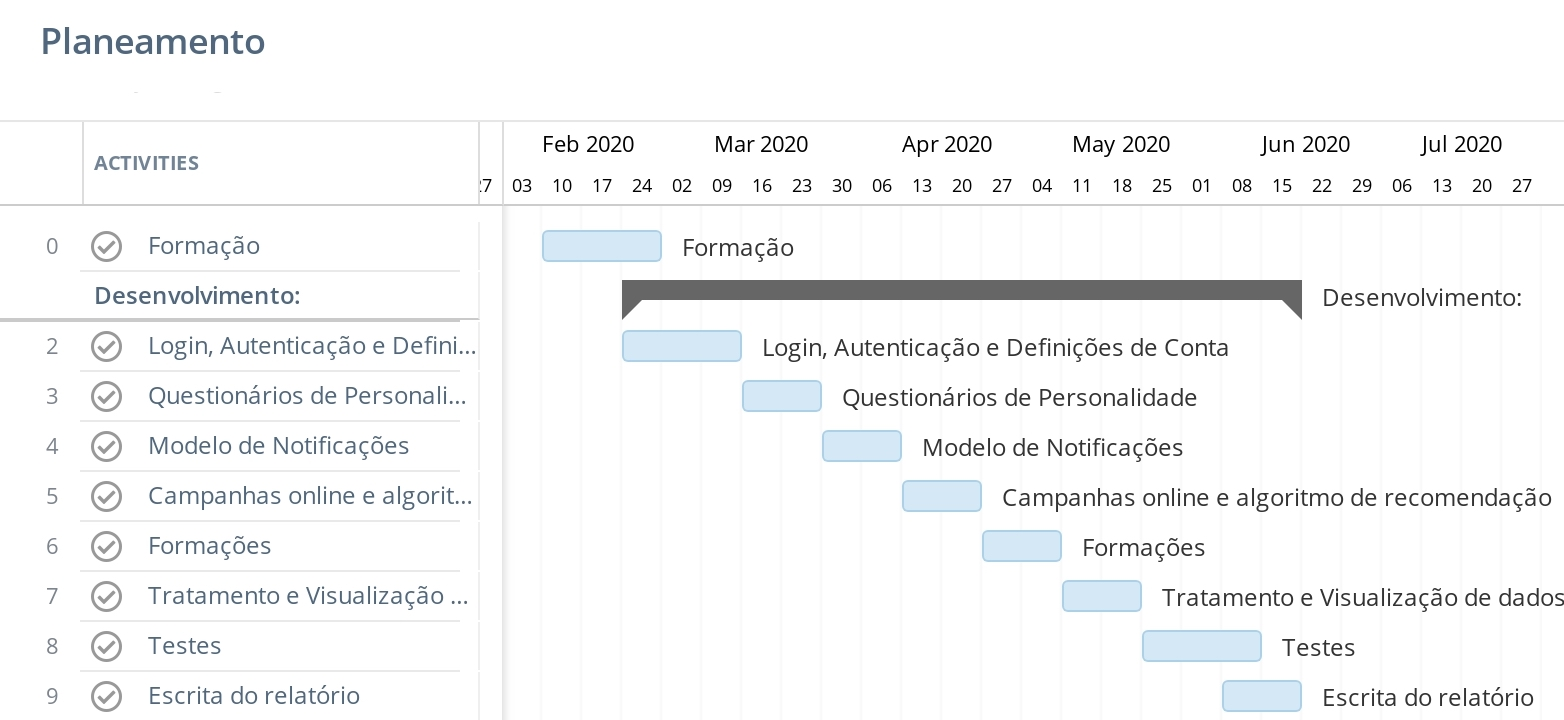
\includegraphics[width=1\textwidth]{img/gantt/semestre2.jpeg}
		\caption{Diagrama de Gantt - Planeamento do 2º semestre}
		\label{fig:gantt2}
	\end{center}
\end{figure}

Representado na Figura \ref{fig:gantt2} temos o plano de estágio relativo ao segundo semestre. A fase de implementação divide-se em várias \textit{Sprints}, que serão detalhadas no Capítulo \ref{sec:sprints}.



MOTRAR GRÁFICO COM O TEMPO REAL DAS SPRINTS E EXPLICAR O PORQUE!!!!


\section{Analise se Riscos}
\label{analiseriscos}
%-------------------------------------------------------------------------------------------------
\blankpage
%-------------------------------------------------------------------------------------------------

\glsresetall



